\documentclass[10pt,a4paper]{article}
\usepackage[utf8]{inputenc}
\usepackage[francais]{babel}
\usepackage[T1]{fontenc}
\usepackage{amsmath}
\usepackage{amsfonts}
\usepackage{amssymb}
\usepackage{graphicx}
\usepackage{epstopdf}
\usepackage{url}
\usepackage{fancyhdr}
\pagestyle{fancy}
\usepackage{cite}
\usepackage{algorithm}
\usepackage{algpseudocode}
\usepackage{algorithmicx}


\renewcommand{\algorithmicrequire}{\textbf{Input:}}
\renewcommand{\algorithmicensure}{\textbf{Output:}}



\renewcommand{\headrulewidth}{1pt}
\fancyhead[R]{} 
\fancyhead[L]{\textit{\leftmark}}

\title{Projet MDI343 \\
Apprentissage profond, réseau de neurones, \emph{etc.}}
\author{Antoine BIARD \& Vincent BODIN}
\date{}


\begin{document}
\maketitle

\hrulefill
\vspace{2cm}
\renewcommand{\abstractname}{Résumé}
\begin{abstract}
Ce projet s'attelle à la question de la représentation des données en \emph{machine learning}. Ces représentations, utilisées ensuite par l'algorithme de décision - régression logistique, SVM... - jouent un rôle primordial car porteuses de l'information. A la méthode classique de création de \emph{features} par des connaissances \emph{a priori}, on oppose des méthodes d'extraction de représentation par des structures dites profondes. Notre projet a consisté essentiellement en deux parties : une première partie de compréhension et d'étude des principales méthodes, et une seconde d'implémentation et de test sur quelques unes de ces méthodes (RBM, MLP, DBN).
\end{abstract}

\newpage
\tableofcontents
\newpage

\section{Introduction : de l'importance de la représentation des données}

Ces dernières années se sont imposées massivement des méthodes dites d'apprentissage profond - \emph{deep learning} en anglais. La communauté scientifique a accru son intérêt en la matière au vue de leurs résultats, dans des domaines aussi variés que la vision par ordinateur ou la reconnaissance vocale. Atteignant souvent des performances au moins équivalentes à l'état de l'art, de nombreux algorithmes de type profond ont été créés pour tenter d'améliorer encore la représentation.

La représentation est une clef fondamentale dans l'élaboration d'un processus d'intelligence artificielle, en ceci qu'elle concentre l'information des données. On distingue en effet une première étape d'apprentissage de la représentation, puis une seconde d'apprentissage, à partir de cette représentation, d'une décision - pour de la classification par exemple. Les algorithmes effectuant cette dernière tâche sont hautement dépendants des données fournies en entrée. Une amélioration de la représentation entraîne de fait une meilleure performance dans la prise de décision. Nous renvoyons à la deuxième section de \cite{DBLP:journals/corr/abs-1206-5538} pour des quantifications d'amélioration de la performance avec des représentations plus élaborées.

Traditionnellement, les descripteurs - ou encore \emph{features} en anglais - sont extraits de façon dite supervisée à partir des données. Ceci nécessite une connaissance \emph{a priori} dans le domaine, puisque cela requiert souvent une importante étape de traitement des données pour en extraire l'information - citons parmi tant d'autre en vision les points de Harris et les SIFT ou encore le spectrogramme et les \emph{Mel-frequency cepstrum coefficients} en audio. Cela repose sur l'idée que l'homme a la capacité d'extraire et d'organiser l'information intrinsèque des données. Pour autant, dans un cadre d'intelligence artificielle pure, il serait désirable de s'affranchir de cette hypothèse et d'implémenter des algorithmes capables d'apprendre une représentation convenable sans supervision - non-supervisé. En outre, les types de données ayant tendance à devenir de plus en plus variés - image, son, web... - une telle connaissance dans chaque domaine s'avère illusoire et le manque de généralité de ces méthodes se paye dans la nécessité d'expertise dans chaque domaine. Il s'agit d'implémenter des méthodes extrayant des données une représentation abstraite.

Une manière d'atteindre ce but est l'extraction d'une représentation par apprentissage profond - \emph{deep learning}. Une telle représentation s'obtient par l'ajout de couches successives. Une première représentation est obtenue par un processus à partir des données pures, puis cette représentation est elle-même raffinée, et ainsi de suite. Dans l'espoir d'obtenir une représentation abstraite, la non-linéarité devient nécessaire puisque sans elle, l'ajout de deux couches linéaires serait équivalent à une unique couche - le concept de profondeur perdrait sens.

Nous allons par la suite détailler les algorithmes d'apprentissage profond les plus classique, puis nous comparerons les performances de certains d'entre eux. 







\section{Revue élémentaire des méthodes de \emph{deep learning}}

\subsection{Réseau de neurones}

Un réseau de neurone peut être vu comme l'utilisation en série et parallèle plusieurs neurones simples, cf. Fig.(\ref{fig1}). Un neurone est un noeud, avec un certain nombre d'entrée, et une fonction d'activation, disons $\sigma$ - souvent tangente hyperbolique ou une sigmoïde, l'idée étant d'avoir une fonction proche de la fonction seuil, qui donne une activation \emph{soft}. Pour un neurone ayant $p$ entrée, chacun pondéré par un poids $w_i$, et un \emph{offset} b, la sortie du neurone est :
\begin{equation}
h_{w,b}(x)=\sigma(w^Tx)=\sigma\left(\sum_{i=1}^p w_i x_i + b\right)
\end{equation}

Dans le cas d'un réseau de neurones, en utilisant une formule de chaîne où chaque sortie de neurone intermédiaire devient l'entrée du neurone suivant, on obtient un réseau du type de la Fig.(\ref{fig1}). On voit ici apparaître naturellement l'idée de profondeur dans l'apprentissage par accumulation de couche de neurone, bien qu'il s'agisse du modèle le plus basic d'apprentissage profond. La fonction de sortie dépend de tous les paramètres $w,b$ à chaque couche et chaque noeuds. La difficulté majeure dans l'apprentissage profond réside en l'estimation des paramètres optimaux - dans le sens où la sortie est la représentation la plus adéquate.

\begin{figure}[ht!]
\centering
\begin{tabular}{cc}
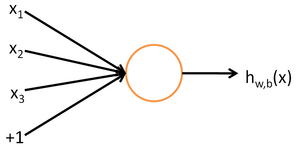
\includegraphics[width = .5\columnwidth]{fig/SingleNeuron.png} &
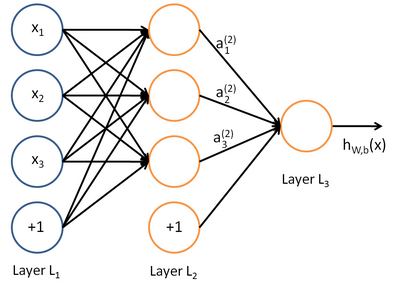
\includegraphics[width = .5\columnwidth]{fig/Network331.png} 
\end{tabular}
\caption{(gauche) Un neurone avec trois entrées $(x_1,x_2,x_3)$ et un \emph{offset} ; (droite) un réseau de neurones de taille $(3,3,1)$ avec des \emph{offset} aux deux premières couches.}
\label{fig1}
\end{figure}


\subsection{Multilayer Perceptron (MLP)}

Le second modèle classique en apprentissage profond est le perceptron multi-couche (MLP). Il s'agit du premier exemple d'algorithme utilisant la méthode dite de \emph{backpropagation}. Bien que peu utilisé seul en pratique, car la fonction d'optimisation n'est pas convexe et il y a de grand risque de trouvé un optimum local et non global, le MLP correspond aux prémisses du \emph{deep learning} et sera réutilisé pour des modèles plus complexes par la suite.

\begin{figure}[ht!]
\centering
\begin{tabular}{cc}
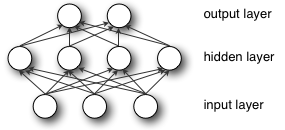
\includegraphics[width = .5\columnwidth]{fig/mlp} &
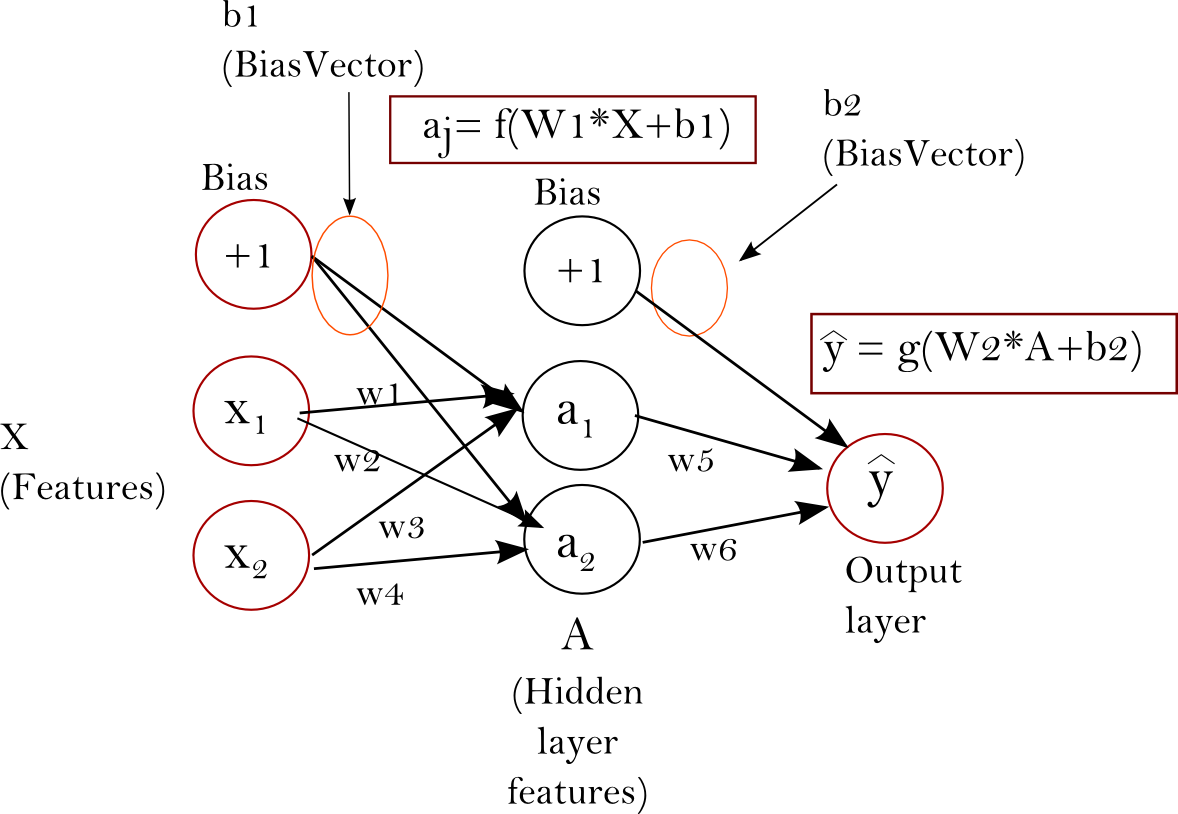
\includegraphics[width = .5\columnwidth]{fig/backprop_notation.png} 
\end{tabular}
\caption{(gauche) Un MLP avec une seule couche de variables cachées ; (droite) structure de MLP avec l'ajout de biais et les notions de poids.}
\label{fig2}
\end{figure}

Le MLP possède une fonction d'activation $\sigma$ - tangente hyperbolique ou la fonction logistique souvent - des noeuds de biais $b$ et des poids $W$ associés à chaque arrête. Pour chaque couche, le paramètre est donc $\theta = (W,b)$, et pour une entrée $x$ de dimension $d$ - \emph{i.e.} $d$ noeuds - la sortie de cette couche est : 
\begin{equation}
s(x) = \sigma(Wx + b)
\end{equation}
Ceci forme un vecteur de taille disons $m$ - sur la Fif.(\ref{fig2}) par exemple pour la première couche $d=3$ et $m=4$ - qui est envoyé comme entrée à la couche suivante. 

La nouveauté du MLP comparé au réseau de neurone réside en la manière d'apprendre l'hyper-paramètre $\theta = (W_1, \cdots, W_p, b_1, \cdots, b_p)$ - $p$ est le nombre de couches. L'algorithme en question sera développé plus tard mais nous en donnons un aperçu. L'initialisation s'effectue classiquement de manière aléatoire - bien que dans le cas du DBN on lui envoie des poids définis en entrée. Dans \cite{GlorotAISTATS2010}, il est expliqué comment tirer les poids initialement. L'algorithme contient ensuite deux étapes :
\begin{description}
\item[Forward pass. ]On part des variables visibles $v$ et on remonte le graphe avec les poids de la structure. On en déduit une représentation.

\item[Backpropagation. ]A partir de cette représentation, on effectue le chemin inverse en descendant le graphe et en comptabilisant les erreurs commises. En comparant les résultats de la descente avec les variables visibles, on peut mettre à jour les poids.
\end{description}
Cela est répété un certain nombre de fois et cette mise à jour par \emph{backpropagation} permet d'obtenir une représentation convenable. Toutefois ceci est très dépendant de l'initialisation. 

Notons que ceci ne fournit qu'une représentation. Pour effectuer une classification, on utilise souvent une base de données étiquetée. Chaque représentation est associée à une étiquette et on se sert des représentations comme \emph{feature} de l'algorithme de décision - régression logistique, SVM...



\subsection{Restricted Boltzmann Machine (RBM)}

\subsubsection{Machine de Boltzmann}

Une machine de Boltzmann est un réseau de variables aléatoires couplées. On se restreint au cas où les données sont binaire, on note les variables visibles $v$ et les cachées $h$. Une machine de Boltzmann est représentée en Fig.(\ref{fig3}) à gauche.

\begin{figure}[ht!]
\centering
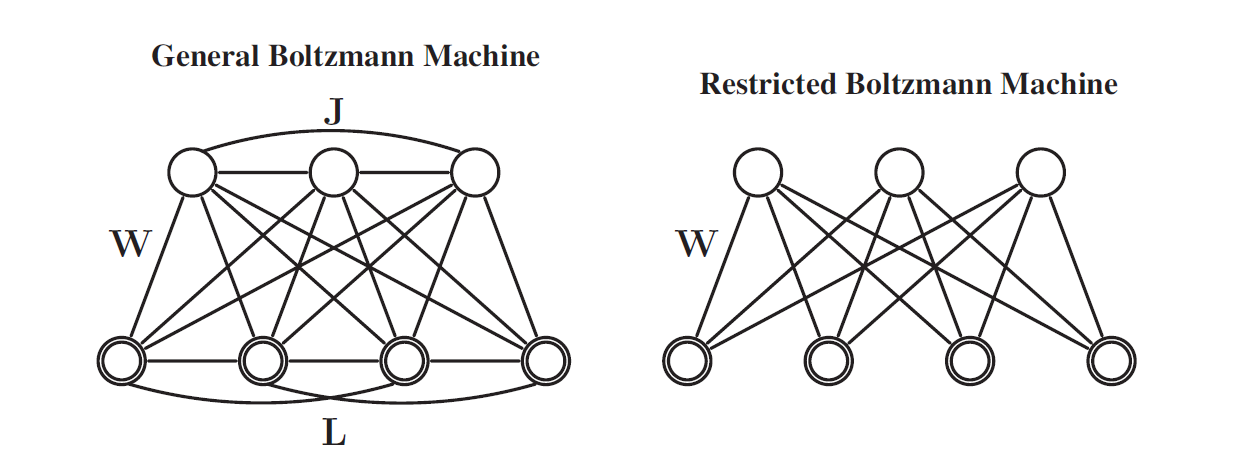
\includegraphics[width = \columnwidth]{fig/boltzmann_machine.png}
\caption{(gauche) Une machine de Boltzmann générale ; (droite) machine de Boltzmann restreinte (RBM).}
\label{fig3}
\end{figure}

L'énergie des états $(v,h)$ prend alors la forme : 
\begin{equation}
E(v,h ; \theta) = -v^TWh - \frac{1}{2}v^TLv - \frac{1}{2}h^T Jh
\end{equation}
(où l'on ne prend pas en compte ici les termes de biais qui correspondent à un recentrage des $(v,h)$). Il s'agit d'un cas de \emph{energy-based models} (EBM). Dans ce cas, la probabilité d'un état $v$ s'écrit : 
\begin{equation}
p(v;\theta) = \frac{1}{\mathcal{Z}}\sum_h e^{-E(v,h;\theta)}
\end{equation}
où $\mathcal{Z} = \sum_{x,h}e^{-E(v,h;\theta)}$ est la fonction de partition. Ces modèles ont la propriété que le gradient de $\log p(v)$ - log-vraisemblance - se décompose en deux termes, une phase positive et une négative. Pour autant la vraisemblance n'est pas calculable car exponentielle à la fois en le nombre de variables cachées et visibles. 



\subsubsection{Restricted Boltzmann Machine}

Comme montré dans la Fig.(\ref{fig3}), un RBM est une machine de Boltzmann où les interactions inter-couches sont gelées. De par la forme de son graphe, le RBM a des propriétés d'indépendances conditionnelles qui rendent l'inférence facile en pratique : 
\begin{equation}
\begin{array}{rll}
p(h|v) & = & \displaystyle \prod_{i} p(h_i|x) \\
p(v|h) & = & \displaystyle \prod_{j} p(x_j|h)
\end{array}
\end{equation}
Par suite on a : 
\begin{equation}
\begin{array}{rll}
p(h_i = 1 |v ) & = & \displaystyle \sigma\left(\sum_j W_{ji}x_j + d_i\right) \\
p(x_j = 1 |h ) & = & \displaystyle \sigma\left(\sum_i W_{ji}h_i + b_j\right)
\end{array}
\end{equation}
où $\sigma$ est la fonction d'activation, et les $(b,d)$ sont les biais. Pour autant, comme la plupart du temps, la fonction de partition reste incalculable en pratique, mais ces formules de factorisation permettent d'effectuer de l'inférence sans avoir à la calculer.

Nous en reparlerons plus en détail dans la partie d'implémentation, mais l'entraînement d'un RBM nécessite d'effectuer des étapes d'échantillonnage - de Gibbs - souvent par des méthodes MCMC. Il existe plusieurs méthodes pour accélérer le processus, nous parlerons de la \emph{Contrastive Divergence} (CD) et du \emph{Stochastic Maximum Likelihood} (SML).

%\part{Hoplaboom}

\section{Iap}

\subsection{Upe}

\subsection{Deep Belief Networks (DBN)}

Un DBN est une structure d'apprentissage de représentation qui consiste en un empilement de RBM. Le premier RBM prend en entrée les variables visibles - données du problème - et, par échantillonnage en extrait un ensemble de variables cachées. Celles-ci sont alors utilisées comme entrée de la seconde couche et ainsi de suite, cf. Fig.(\ref{fig4}). L'entraînement est donc de type \emph{greedy}. Finalement, la probabilité jointe entre $x$ et $h$ s'écrit :
\begin{equation}
p(x, h^1, \cdots, h^l) = \left( \prod_{k=0}^{l-2} p(h^k |h^{k+1}) \right) p(h^{l-1}, h^l)
\end{equation}
avec $x=h^0$. Nous verrons l'implémentation de l'algorithme en détail plus tard. En modèle graphique, cette décomposition s'interprète comme un graphe dont la dernière couche est non-orientée tandis que toutes les précédentes sont des graphes orientés.

L'entraînement du DBN repose en outre sur un \emph{fine-tuning} des paramètres obtenus par apprentissage par couches sur les RBM. Le \emph{fine-tuning} s'effectue soit selon un \emph{proxy} de la log-likelihood - cas non-supervisé - ou d'un critère d'erreur dans le cas supervisé. Nous nous plaçons dans le cas supervisé, et la méthode de classification appliquée est le MLP.

\begin{figure}[ht!]
\centering
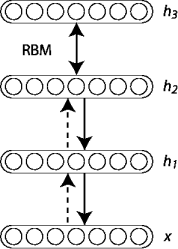
\includegraphics[width = .3\columnwidth]{fig/DBN3.png}
\caption{Un \emph{deep belief network} (DBN), la dernière couche est non orientée, tandis que toutes les autres le sont.}
\label{fig4}
\end{figure}

Nous pouvons donner ici une justification rapide du \emph{pre-training} par couche. Dans le cas de deux couches par exemple, il a été montré \cite{DBLP:bibsonomy_HintonSalakhutdinov2006b} que :
\begin{equation}
\log p(x) = \text{KL}(Q(h^{(1)}|x) \| p(h^{(1)}|x)) + \text{H}_{Q(h^{(1)|x)}} + \sum_h Q(h^{(1)}|x) \left( \log p(h^{(1)}) + \log p(x | h^{(1)}))\right)
\end{equation}
où KL est la divergence de Kulbac-Leibler, H l'entropie, $Q(h^{(1)}|x)$ la distribution \emph{a posteriori} du premier RBM (appris seul) et $p(h^{(1)}|x)$ celle après l'apprentissage entier du DBN. Si l'initialisation est $W^{(2)} = W^{{(1)}T}$ alors $Q(h^{(1)}|x) = p(h^{(1)}|x)$ et la divergence est nulle. Fixer ensuite $W^{(1)}$ et optimiser selon $W^{(2)}$ ne peut qu'augmenter la log-vraisemblance.




\subsection{Deep Boltzmann Machine (DBM)}

Un DBM est une structure profonde qui,  en première approche tout au moins, ressemble fortement à un DBN. De la même manière que le DBN, le DBM extrait une représentation abstraite des données. Également, un faible nombre de données étiquetées est nécessaire à la tâche de classification, ce qui peut être intéressant dans certains cas. Il est dit dans \cite{SalHinton07} que l'inférence dans les DBM est plus robuste que dans les DBN car les entrées ambiguës ont moins d'impact. 

Un DBM est constitué de RBM empilés comme dans le cas des DBN. L'étape de \emph{pre-training} se résume à un entraînement couche par couche - \emph{greedy} - de ces RBM. L'idée pour autant est de modifier un peu cette étape pour éviter le double passage quand on fait les étapes de haut vers le bas et bas vers le haut. Ainsi, pour le niveau le plus bas - plus bas RBM - les entrées sont doublées avec les poids visibles-cachés inchangés, cf. Fig.(\ref{fig5}). Une étape d'évaluation du DBM basé sur des méthode de Monte Carlo - \emph{Annealed Importance Sampling} - a ensuite lieu. Finalement, on termine comme dans le cas du DBN par du \emph{fine-tuning} avec un MLP par exemple - qui converti la représentation en étiquette.

\begin{figure}[ht!]
\centering
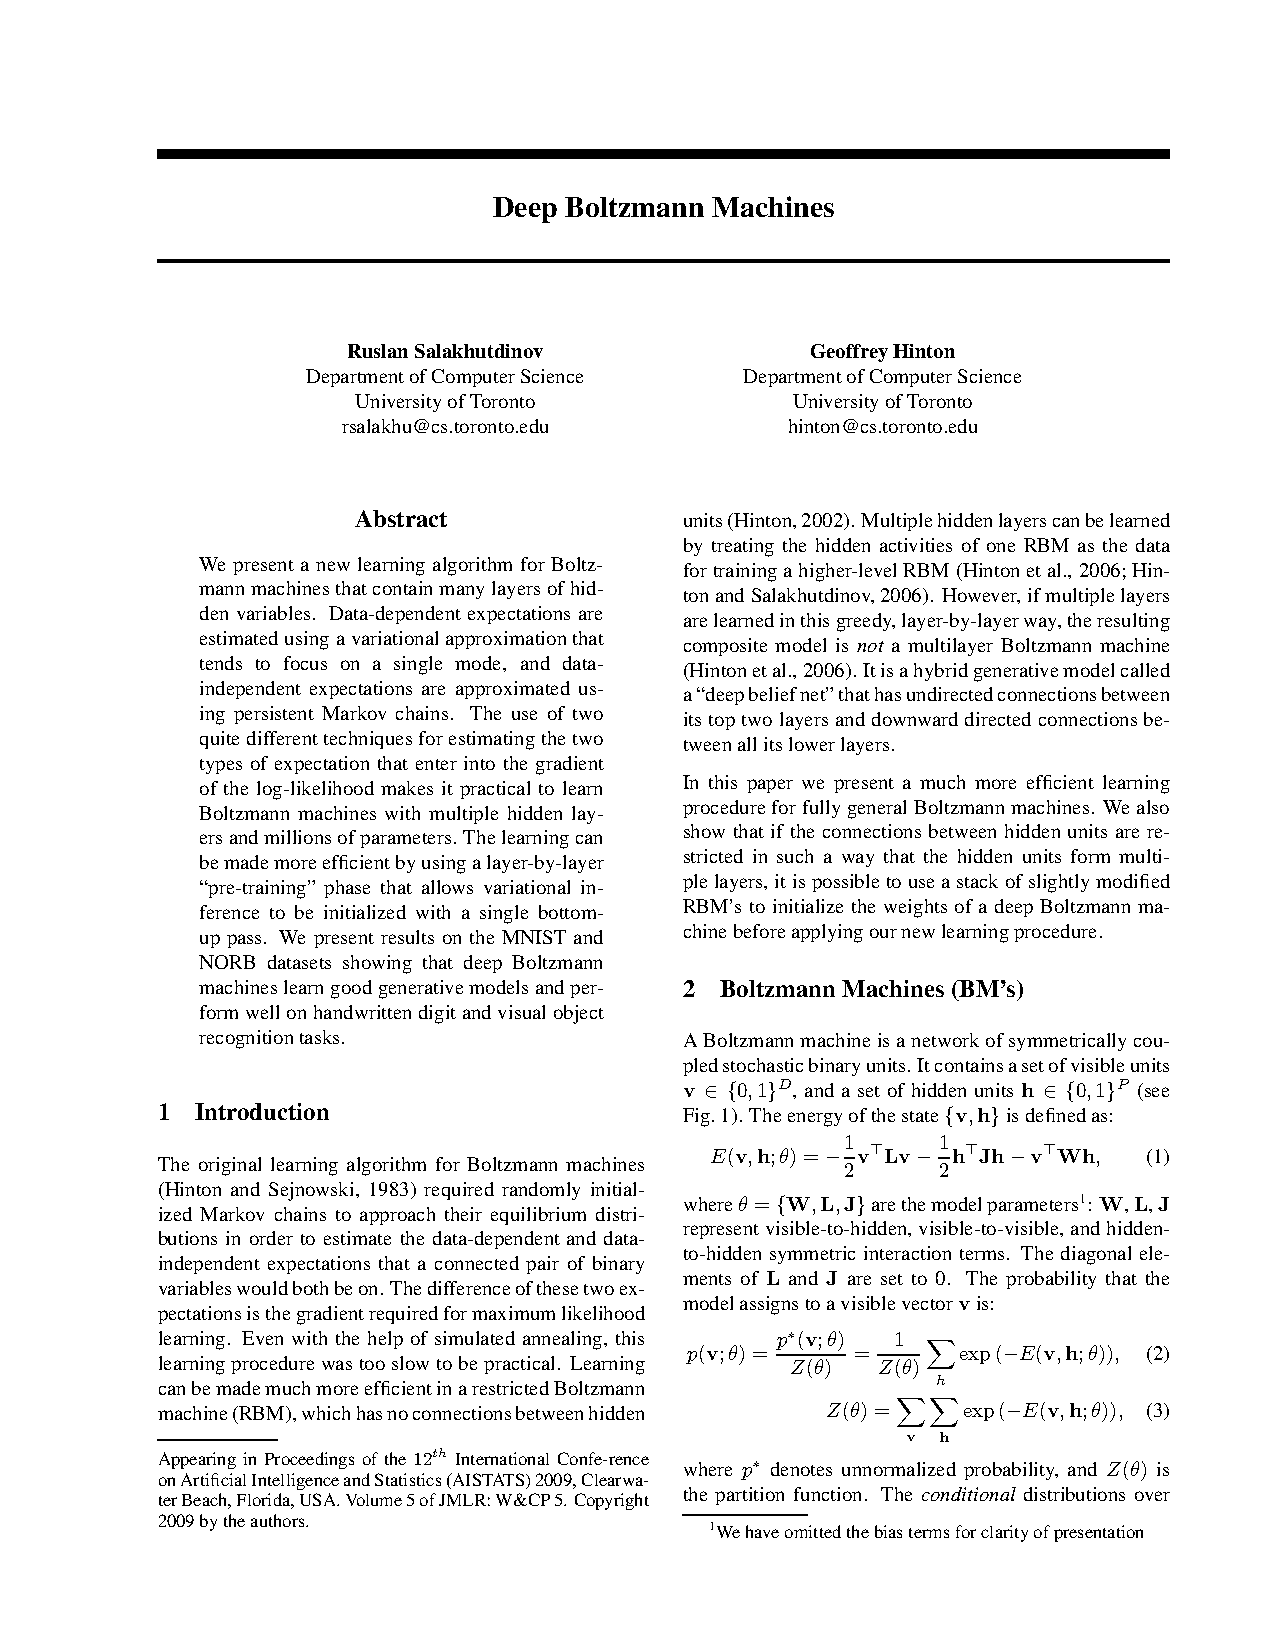
\includegraphics[width = \columnwidth]{fig/dbm.png}
\caption{(extrême gauche) Un DBN avec sa dernière couche non orientée ; (gauche) graphe de DBM, toutes les couches sont non orientées ; (droite) \emph{pre-training} des RBM couche par couche ; (extrême droite) composition des couches pour former le DBM.}
\label{fig5}
\end{figure}




\subsection{Auto-Encoder}

La dernière méthode que nous présentons succinctement est celle des \emph{auto-encoder}. Partant d'un ensemble d'apprentissage $x^{(t)}$ on extrait des descripteurs $h^{(t)}$ à l'aide d'une fonction paramétrique $f_{\theta}(x)$. Une autre fonction $g_{\theta}$ est appelé le décodeur et permet de faire la transformation inverse, $r=g_{\theta}(h)$ s'appelle la reconstruction. Une erreur de reconstruction est définie $L(x^{(t)}, r)$. Finalement, l'entraînement de l'auto-encodeur consiste à trouver le paramètre $\theta$ vérifiant :
\begin{equation}
\mathcal{J}_{\text{DAE}}(\theta) = \sum_{t} L(x^{(t)}, g_{\theta}(f_{\theta}(x^{(t)})))
\end{equation}
La forme la plus usuelle pour les fonctions $f_{\theta}$ et $g_{\theta}$ est : 
\begin{equation}
\begin{array}{rll}
f_{\theta}(x) & = & s_f(b + Wx) \\
g_{\theta}(h) & = & s_g(d + W'h)
\end{array}
\end{equation}
où typiquement $s_f$ et $s_g$ sont des sigmoïdes ou des tangentes hyperboliques. 







%%%%%%%%%%%%%%%%%%%%%%%%%%%% MLP %%%%%%%%%%%%%%%%%%%%%%%%%%%%


\subsubsection{Implémentation du MLP}

Nous avons implémenter l'algorithme le plus classique dans le cas de l'entraînement du MLP : la \emph{backpropagation}. Cet algorithme se décompose en deux étape, une première de propagation, et une seconde de mise à jour des poids. 

\paragraph{Initialisation. }L'initialisation est cruciale dans ces algorithmes de \emph{backpropagation}. De plus, comme nous allons utiliser le MLP dans le cas de poids initialisés par empilement de RBM - pour le DBN - notre implémentation doit prendre en compte deux possibilités. Soit on lui envoie les poids, soit on utilise le MLP à part entière et dans ce cas là les poids doivent être initialisés. Dans \cite{GlorotAISTATS2010}, il est expliqué que les poids doivent vérifiés (si $n_1$ et $ n_2$ indiquent le nombre d'éléments au couches d'entrées et de sorties respectivement) : 
\begin{equation}
\begin{array}{ll}
\displaystyle \left[ - \sqrt{\frac{6}{n_1+n_2}} , \sqrt{\frac{6}{n_1+n_2}}\right] & \text{pour activation en} \tanh \\
\displaystyle \left[ - 4\sqrt{\frac{6}{n_1+n_2}} , 4\sqrt{\frac{6}{n_1+n_2}}\right] & \text{pour activation en sigmoïd} 
\end{array}
\end{equation}


\paragraph{Propagation. }La propagation correspond à une étape de montée du graphe pour générer les sorties correspondantes puis à une étape de descente qui génère des $\delta$. Ceci nécessite une étiquette $y$ que l'on compare avec la variable cachée finale $h$ - éventuellement ceci peut être vectoriel. Nous verrons dans Alg.(\ref{algoVince}) l'algorithme précisément. 

\paragraph{Mise à jour des poids. }Pour chaque synapse on met à jour les poids avec les $\delta$ calculé par propagation. Ceci nécessite un paramètre, le \emph{learning rate} qui influence fortement la qualité et la vitesse de l'apprentissage. \\


\begin{algorithm}[ht!]
\caption{Entraînement du Multi-Layer Perceptron (MLP)}
\label{algoVince}
\begin{algorithmic}
\Require $X$ : matrice d'entrainement, $y$ : étiquettes d'entraînement, $l_r$ : \emph{learning\_rate}, $epochs$ : nombre d'itérations, ($W$ : liste de matrice de poids)

\Ensure $W$ : liste de matrice de poids optimaux

\State Rajoute une colonne de 1 à la matrice $X$ (biais),
\For{$k\in\texttt{range}(epochs)$}
	\State $\texttt{states} = [X[i]]$ où $i$ est un indice de ligne tiré aléatoirement,
	
	\For{$j$ monte le graphe (propagation)}
		\State $\texttt{states.append(states}[j]\cdot W[j])$
	\EndFor
	
	\State \texttt{error} = y[i] - \texttt{states}[end]
	\State $\delta = [\texttt{error}*\partial\sigma(\texttt{states}[end])]$
		
	\For{$j$ descend le graphe (backpropagation)}
		\State $\texttt{deltas.append((deltas}[end]\cdot W[j]^T) \times \partial \sigma(\texttt{states}[j]))$
	\EndFor
	\State $\delta .$revese()
	
	\For{$i$ monte le graphe (mise à jour)}
		\State W[i] += $l_r(\texttt{vecteur de nombres de composant}^T\cdot \delta)$
	\EndFor
\EndFor
\end{algorithmic}
\end{algorithm}

La prédiction dans le cas d'un MLP consiste uniquement à, une fois les poids établis, utiliser les données et monter le graphe pour retrouver leur représentation. En ce sens, on considère un MLP comme un pur outils de représentation - vision non-paramétrique. On peut toutefois lui rajouter une régression logistique à l'issue - lorsque l'on dispose de données supervisées - qui permet d'en faire un outils de classification supervisée.  


%%%%%%%%%%%%%%%%%%%%%%%%%%%%%%%%%%%%%%%%%%%%%%%%%%%%%%%%%%%%%


\newpage

\bibliographystyle{unsrt}
\bibliography{biblio}

\end{document}